\documentclass[../main.tex]{subfiles}

\begin{document}

\chapter[Temperature and Ice]{The Impact of Temperature on Antarctic Ice}
\label{chap:temp_and_ice}

The variable which we found had the largest impact on the behaviour of ice in Antarctica is temperature. This follows naturally from the basic thermodynamics of phase change. As the temperature increases we see lower concentrations of sea ice, and as the temperature increases we see lower concentrations of sea ice. The extent of this relationship will be explored in detail in this chapter. We will first look at the relationship through density plots \textcolor{red}{Check name of plots}. Before calculating correlations and looking at the similarities and differences of the two different variables.

For the purpose of this chapter, when we use temperature we will use \gls{skt} as discussed before \textcolor{red}{Write up different temperatures.}

\section{Temperature and ice anomalies}
In this chapter we will be looking at both anomalous and raw datasets. We define anomalous values as follows.

Let $y(t,x,y)$ be our time-series of measured values. $x$ and $y$ are spatial coordinates. For the purposes of this exercise the spatial coordinates are arbitrary as we apply the calculations separately for each time-series found at each location. For each month we take the average value of our variable $y$ and subtract that from every instance of that month in the time-series. In the case of annual data there is only one mean value for each time-series. In order to demonstrate the spatial variability in the data which is lost by finding the anomalous values, we have plotted the mean value for the variables used in this chapter below (Figure \ref{fig:mean_distributions}).

Below in figure \ref{fig:mean_distributions} we have plotted the mean values of \gls{sic}, \gls{skt}, and \gls{lilwet}.


\begin{figure}[ht!]
\centering
\begin{subfigure}[ht!]{0.49\textwidth}
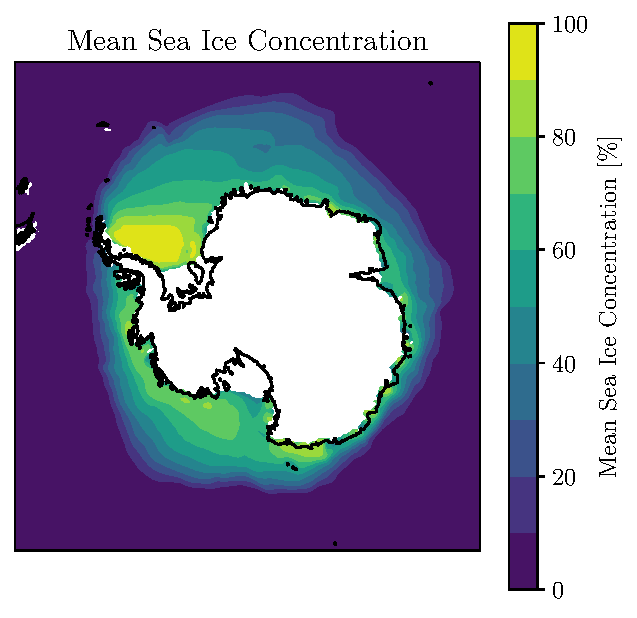
\includegraphics[width=0.9\textwidth]{images/week8/hres/mean_sic_distribution}
\caption{Mean \gls{sic} over Antarctica.}
\end{subfigure}
\begin{subfigure}[ht!]{0.49\textwidth}
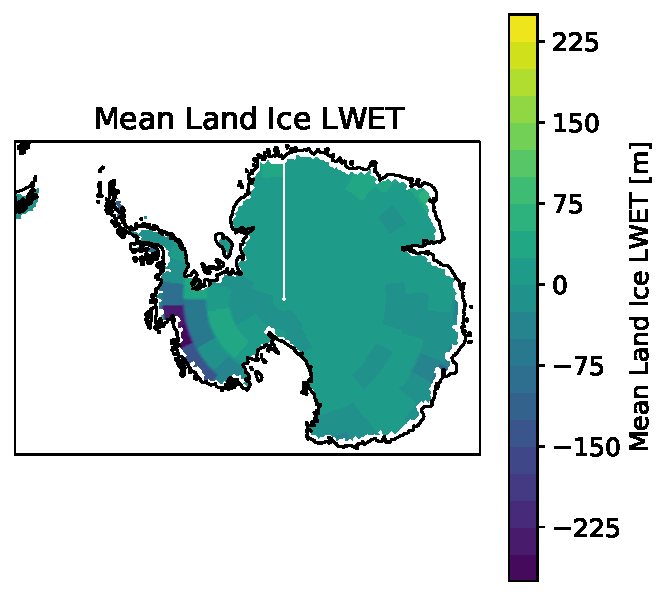
\includegraphics[width=0.9\textwidth]{images/week8/hres/mean_lic_distribution}
\caption{Mean \gls{lilwet} over Antarctica.}
\end{subfigure}
\begin{subfigure}[ht!]{0.49\textwidth}
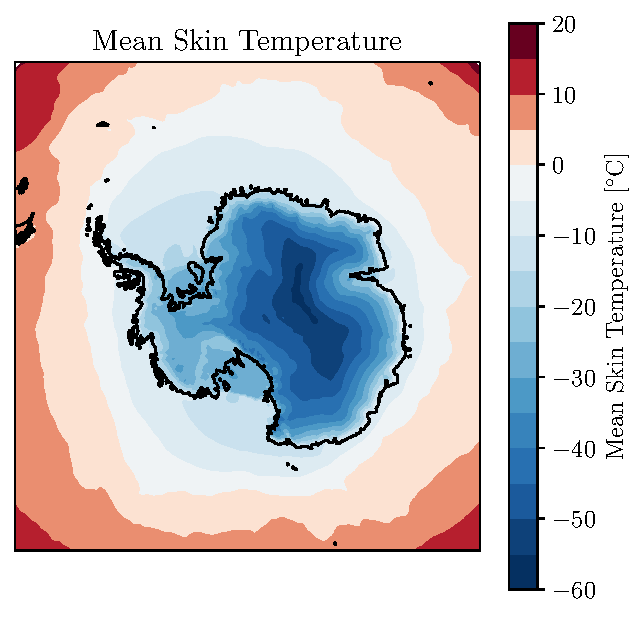
\includegraphics[width=0.9\textwidth]{images/week8/hres/mean_skt_distribution}
\caption{Mean \gls{skt} over \\ Antarctica.}
\end{subfigure}
\caption{Spatial distributions of the mean values of different variables used in this chapter.}
\label{fig:mean_distributions}
\end{figure}

Looking at these plots, it is worth noting that the mean \gls{skt} over the ocean is around 0 degrees close to Antarctica, and so in this region we expect to see a large amount of melting and refreezing of ice as the temperature shifts above and below the freezing point, whereas over land, the temperature tends to be much colder. As such we don't expect temperatures to be above freezing often, so while temperature change may be related to variability in ice change it will not necessarily be the predominant driving factor. 


\section{Visually comparing temperature and ice}
Before we get into any aggregation let's compare the amount of ice at each time and space coordinate in our dataset with the temperature at the associated grid point. For this we will plot 4 2-dimensional histograms of 


The top row contains all the gridpoints over land, the corresponding ice values being \gls{lilwet}. And the row subplot contains all the gridpoints over the sea, with Sea ice concentration (SIC) plotted on the y-axis. The left column contains the raw values for each measurement and the right column has the anomalous values where the mean value of each variable is removed for each spatial location. (The values for this is plotted below).
\begin{figure}[ht!]
    \centering
    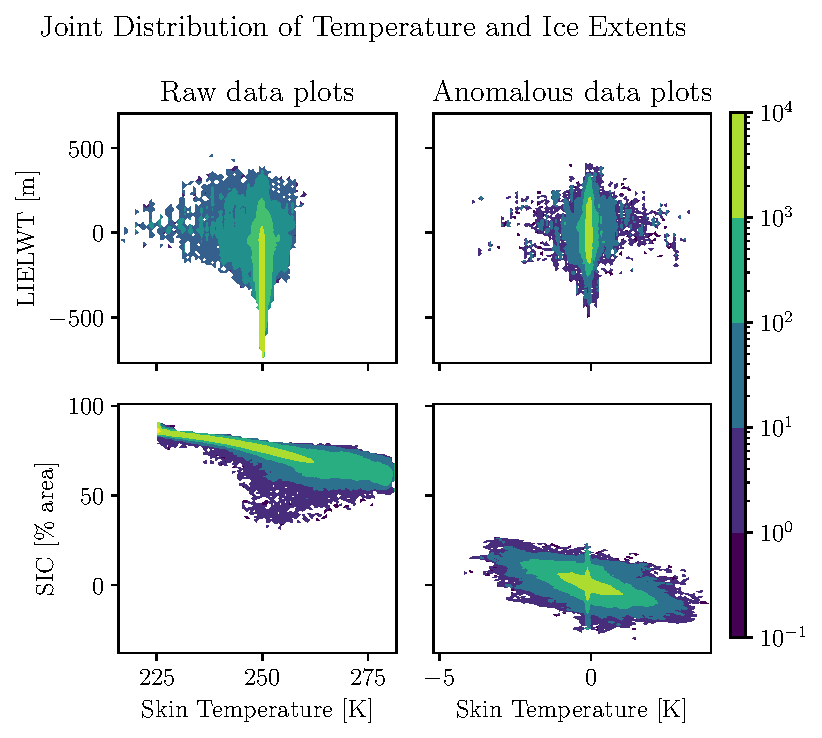
\includegraphics{images/week8/hres/distribution_of_temperature_ice_both_raw_and_anomalous}
    \caption{Distribution of \gls{skt} against ice. Colour represents the number of data points in our dataset with a given histogram box of temperature and ice amounts.}
    \label{fig:joint_distribuition_temp_ice}
\end{figure}

This plot (Figure \ref{fig:joint_distribuition_temp_ice}) tells us an interesting story. For sea ice, we can observe a significant relationship between \gls{skt} and \gls{sic}. This relationship matches with our intuition, which is great. However land ice doesn't exhibit the same strong relationship as sea ice. This is interesting as it suggests that it is driven by a different set of processes. We will have to be careful about this in our ongoing analysis. The anomalous plots tell us a similar story in regards to the relationship between the two variables, however as the overall shape for both land and sea ice plots changed, we expect there to be some spatial variation in how we see the relationship between ice and temperature expressed.

One thing we need to remember with this plot is that it will be exhibiting some spatial bias because some locations will have higher values of ice and lower temperatures. Additionally these plots only contain data points from 2002 because the land ice data only has values from then due to it being based on an later mission. 

We can learn more about this relationship by looking at the spatial and temporal variability and trends for each of the variables.

\section[Spatial distribution of trends]{Spatial distribution of trends in Antarctic ice and temperature}
Our next step in unpacking the relationship between ice in Antarctica and temperature is to look at the trends we see in the different variables


\begin{figure}[ht!]
\centering
\begin{subfigure}[ht!]{0.49\textwidth}
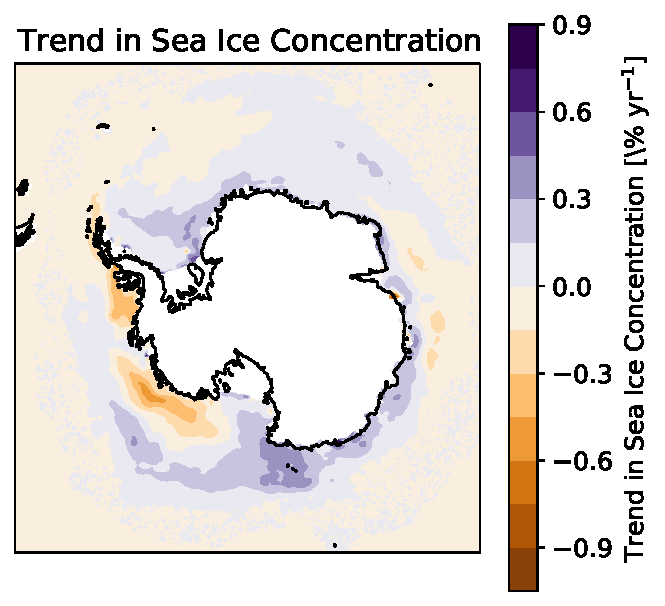
\includegraphics[width=\textwidth]{images/week8/hres/trend_sic_distribution}
\caption{Distribution of trends in \gls{sic} over Antarctica.}
\end{subfigure}
\begin{subfigure}[ht!]{0.49\textwidth}
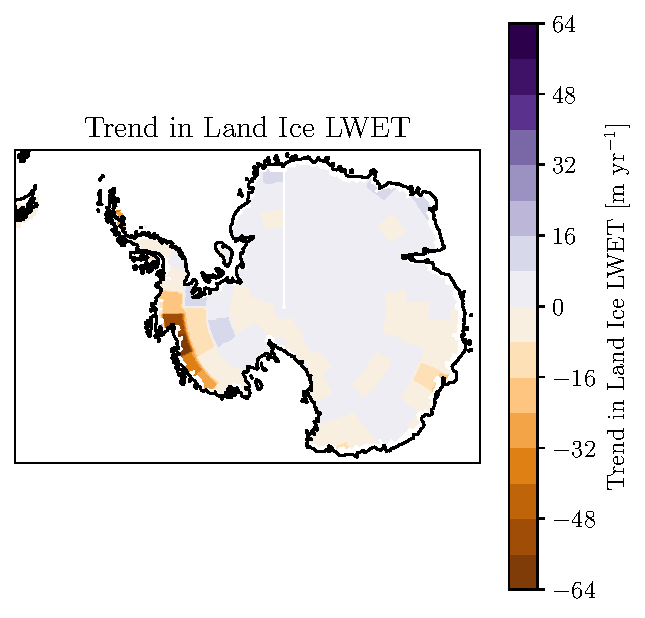
\includegraphics[width=\textwidth]{images/week8/hres/trend_lic_distribution}
\caption{Distribution of trends in Land Ice Liquid Water Equivalent Thickness over Antarctica.}
\end{subfigure}
\begin{subfigure}[ht!]{0.49\textwidth}
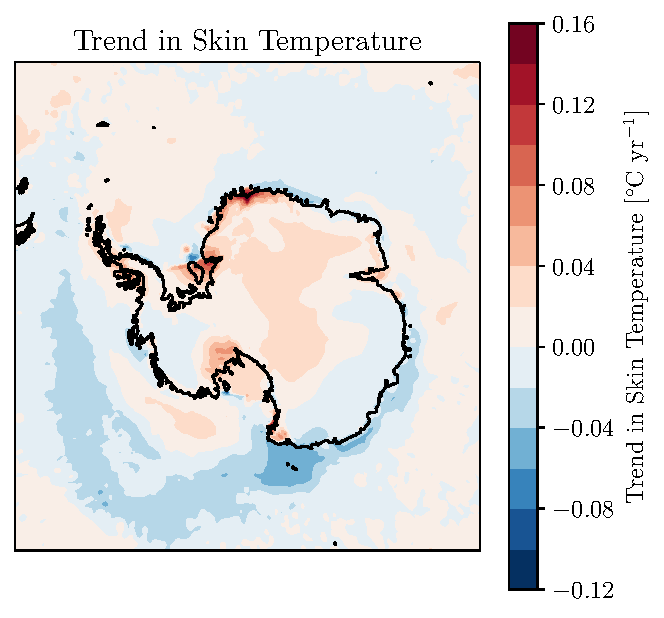
\includegraphics[width=\textwidth]{images/week8/hres/trend_skt_distribution}
\caption{Distribution of trends in \gls{skt} over Antarctica.}
\end{subfigure}
\caption{Spatial distributions of the mean values of different variables used in this chapter.}
\label{fig:trend_distributions}
\end{figure}

Looking at these plots (Figure \ref{fig:trend_distributions}) we can see a clear similarity between the trends in \gls{sic} and \gls{skt}, the regions to the left of the Antarctic Peninsular (Bellingshausen and Amundsen Seas) with decreasing \gls{sic} appear to correspond with an increase in temperature over our time period.
We notice that
To get a better understanding of how good this relationship is we will need to do further analysis (see section \ref{sec:correlations_temp_ice} and \ref{sec:regressions_temp_ice}). Before doing that however, we should look at the temporal variability in our variables to see if there are any notable similarities or differences.

\section{Temporal variability of Antarctic ice and temperature}
Before looking at land and sea ice on the shorter timescale, let's look at the temporal variability of sea ice and different temperatures over our entire time period from 1979 to 2019. This is plotted below in figure \ref{fig:timeseries_seaice_temperature_longterm}. Both time-series were generated by first averaging annually, then removing the mean value at each grid point, then aggregating (by sum in the first plot, by mean in the second). Any and all aggregations are area adjusted to account for the spatial variability of grid size. Linear trend lines have been plotted with each time-series.
\begin{figure}[ht!]
    \centering
    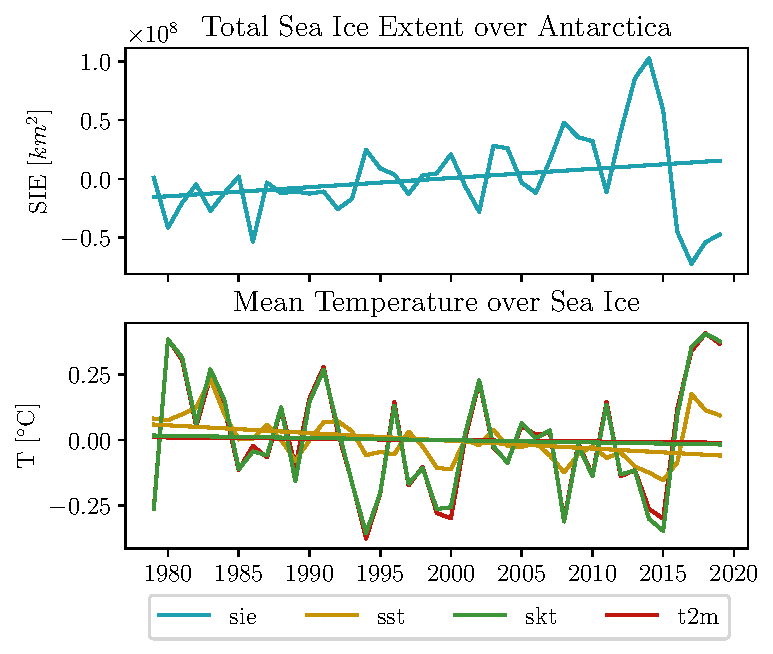
\includegraphics{images/week8/hres/seaice_temperature_timeseries}
    \caption{Time-series for the total \gls{sie} over Antarctica and the mean temperature over sea ice from 1979 to 2019. }
    \label{fig:timeseries_seaice_temperature_longterm}
\end{figure}
Looking at figure \ref{fig:timeseries_seaice_temperature_longterm} the first thing to note is that while we see an increase in \gls{sie} over time, the mean temperatures above ice do not have much of a gradient if any. \gls{sst} does have a negative gradient, however that may be due to its minimum temperature being set to -1.65 $^\circ$C when covered with ice. When we see more ice we expect the average \gls{sst} to decrease because the sea surface will spend more time in a year at its minimum temperature.

Despite the lack of trend in temperatures, we should note that there is a potential relationship between the variability of temperature and \gls{sie}. We often see peaks in temperature at the same time as dips in \gls{sie}, and conversely dips in temperature when we see peaks in \gls{sie}. This fits with the distribution plots (see figure \ref{fig:joint_distribuition_temp_ice} above) but will require a more rigurous statistical analysis to confirm.

We should also acknowledge the difference between \gls{sst} and the other temperature variables. As discussed in greater detail in chapter \ref{chap:data} \textcolor{red}{check this}, \gls{sst} is the estimated temperature at the sea's surface underneath the ice, whereas \gls{skt} and \gls{t2m} are values for estimated temperature above any sea ice, and as such we expect \gls{sst} to exhibit less variability than the other measures of temperature whilst having similar patterns of variability. This is what we observe in figure \ref{fig:timeseries_seaice_temperature_longterm}. 

Now let's consider our shorter timescale (2002-2019) and look at the temporal variability of land ice, sea ice and temperature. This is plotted in figure \ref{fig:timeseries_seaice_temperature_shortterm}. All time-series were generated by first averaging annually, then removing the mean value at each grid point, then aggregating (by sum for ice, by mean for temperature). Any and all aggregations are area adjusted to account for the spatial variability of grid size. Linear trend lines have been plotted with each time-series.
\begin{figure}[ht!]
    \centering
    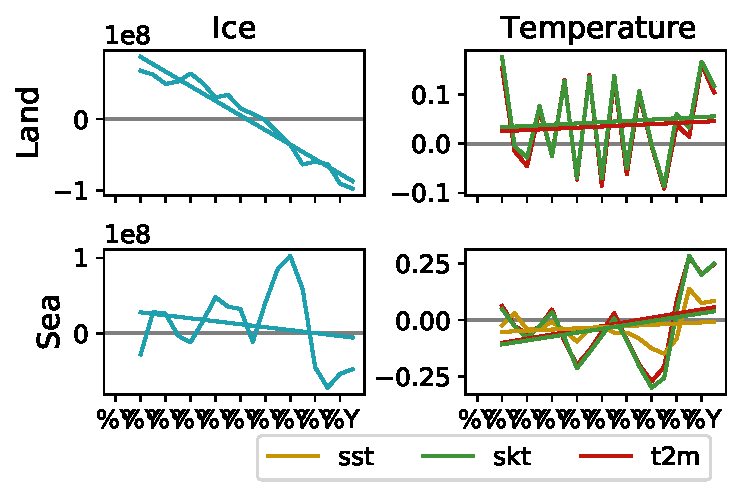
\includegraphics{images/week8/hres/six_timeseries}
    \caption{Time-series for the Ice and temperature quantities 2002 to 2019. The top row contains values over land, the bottom row contains values over the sea. The left column contains Ice variables (Land Ice Liquid Water Equivalent and Sea Ice Extent), and the second column contains plots for temperature. }
    \label{fig:timeseries_seaice_temperature_shortterm}
\end{figure}

\section{Correlations}
\label{sec:correlations_temp_ice}

\begin{figure}[ht!]
\centering
\begin{subfigure}[ht!]{0.49\textwidth}
\centering
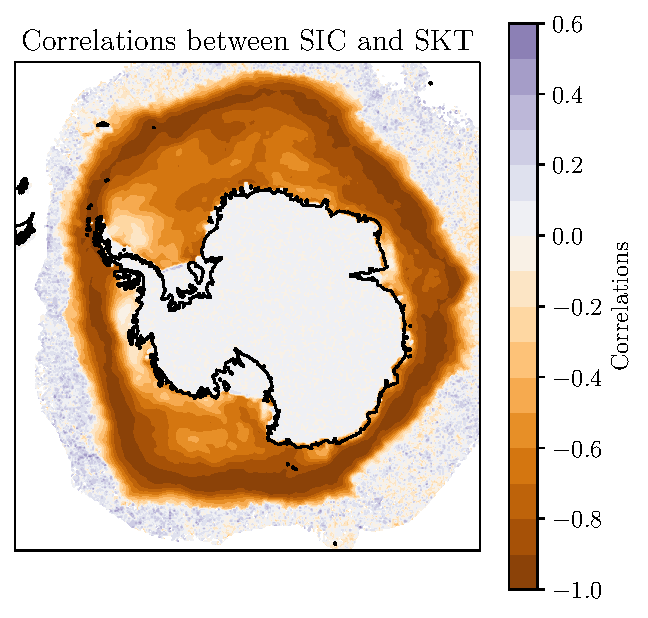
\includegraphics[width=0.9\textwidth]{images/week8/hres/corr_sic_skt_longterm_spatial}
\caption{Spatial distribution of correlations of \gls{sic} and \gls{skt}.}
\end{subfigure}
\begin{subfigure}[ht!]{0.49\textwidth}
\centering
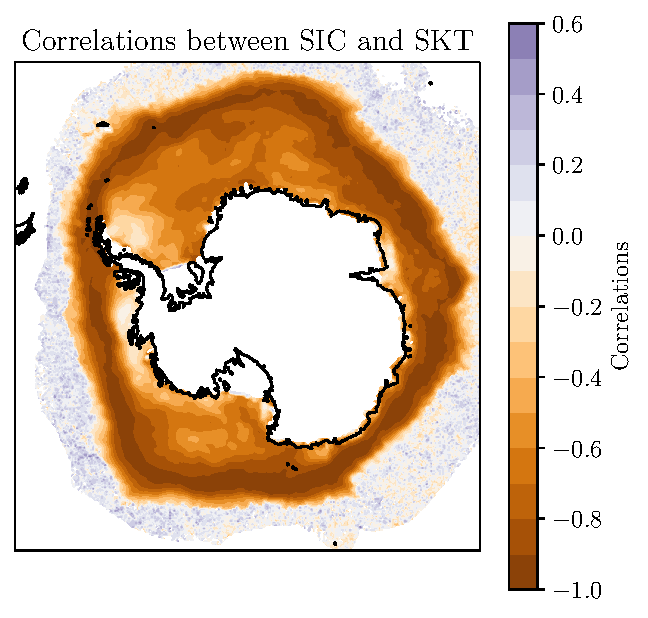
\includegraphics[width=0.9\textwidth]{images/week8/hres/corr_sic_skt_longterm_spatial_anmomalous}
\caption{Spatial distribution of correlations of anomalous \gls{sic} and \gls{skt}.}
\end{subfigure}
\begin{subfigure}[ht!]{0.49\textwidth}
\centering
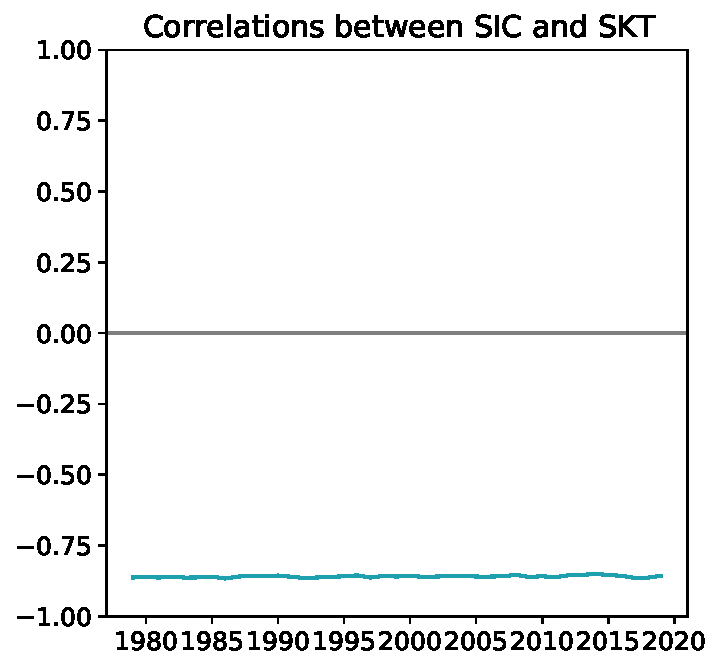
\includegraphics[width=0.9\textwidth]{images/week8/hres/corr_sic_skt_longterm_temporal}
\caption{Temporal distribution of correlations of \gls{sic} and \gls{skt}.}
\end{subfigure}
\begin{subfigure}[ht!]{0.49\textwidth}
\centering
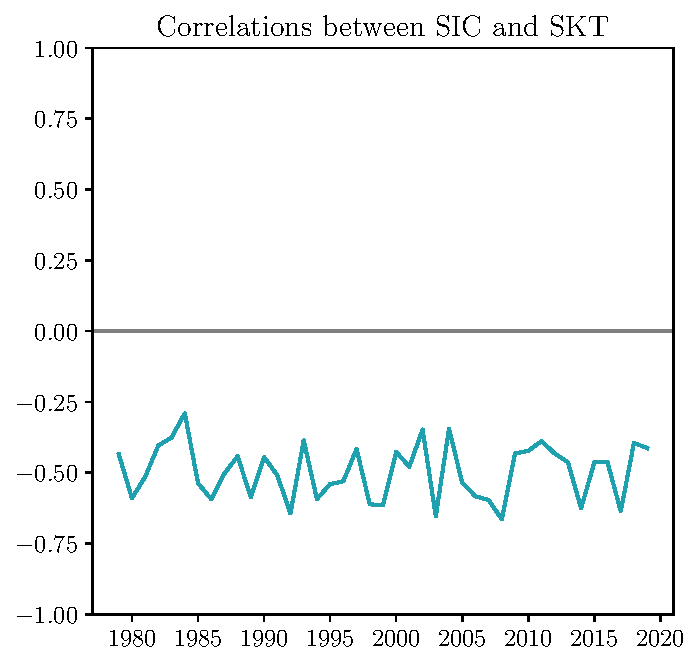
\includegraphics[width=0.9\textwidth]{images/week8/hres/corr_sic_skt_longterm_temporal_anmomalous}
\caption{Temporal distribution of correlations of anomalous \gls{sic} and \gls{skt}.}
\end{subfigure}
\caption{Correlations between \gls{sic} and \gls{skt}. The left column contains correlations for raw data time-series and the right column contains the correlations for anomalous time-series. The top row contains correlations for individual time series. The bottom row contains pattern correlations between the two variables and how that changes over time.}
\label{fig:correlation_between_SIC_and_SKT.}
\end{figure}

\begin{figure}[ht!]
\centering
\begin{subfigure}[ht!]{0.49\textwidth}
\centering
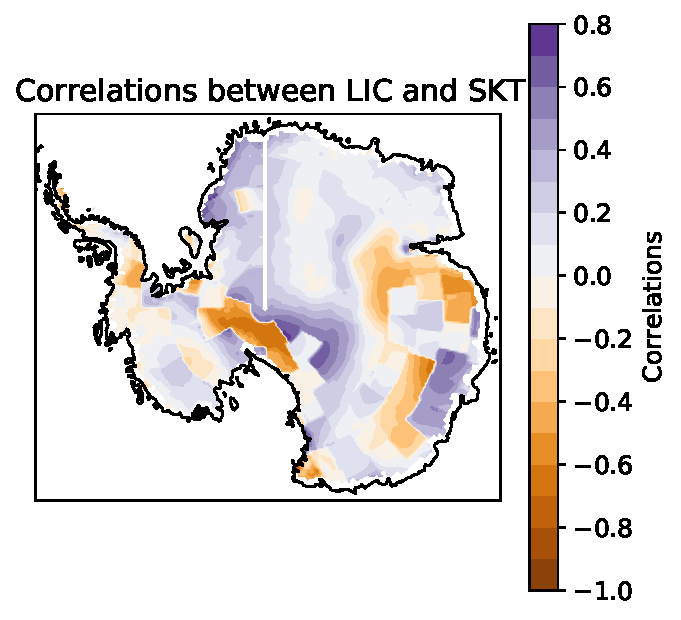
\includegraphics[width=0.9\textwidth]{images/week8/hres/corr_lic_skt_shortterm_spatial}
\caption{Spatial distribution of correlations of \gls{lilwet}  and \gls{skt}.}
\end{subfigure}
\begin{subfigure}[ht!]{0.49\textwidth}
\centering
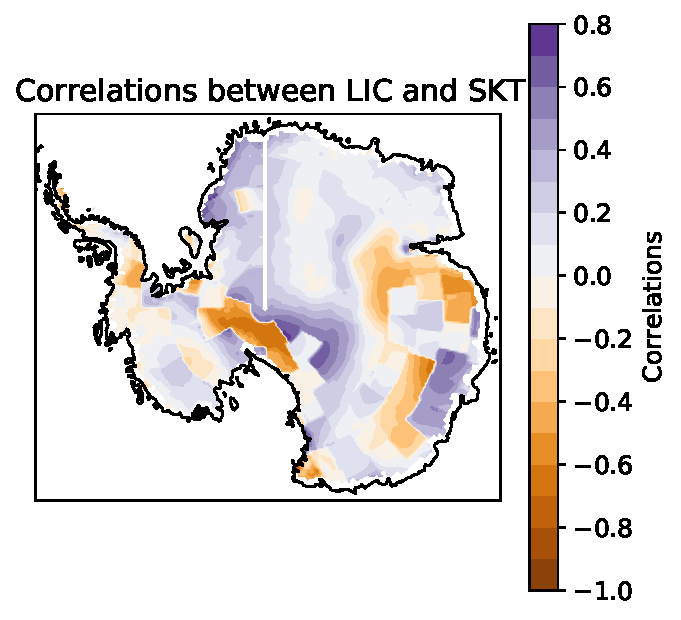
\includegraphics[width=0.9\textwidth]{images/week8/hres/corr_lic_skt_shortterm_spatial_anmomalous}
\caption{Spatial distribution of correlations of anomalous \gls{lilwet}  and \gls{skt}.}
\end{subfigure}
\begin{subfigure}[ht!]{0.49\textwidth}
\centering
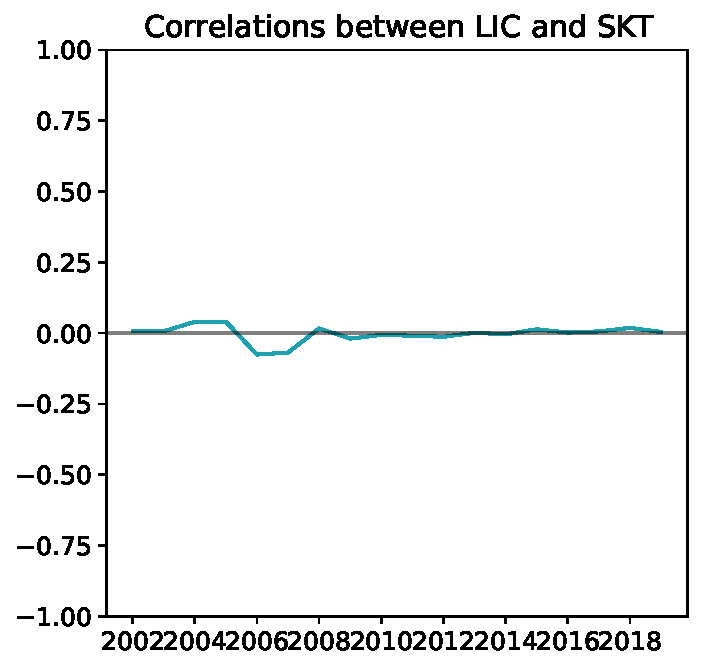
\includegraphics[width=0.9\textwidth]{images/week8/hres/corr_lic_skt_shortterm_temporal}
\caption{Temporal distribution of correlations of \gls{lilwet}  and \gls{skt}.}
\end{subfigure}
\begin{subfigure}[ht!]{0.49\textwidth}
\centering
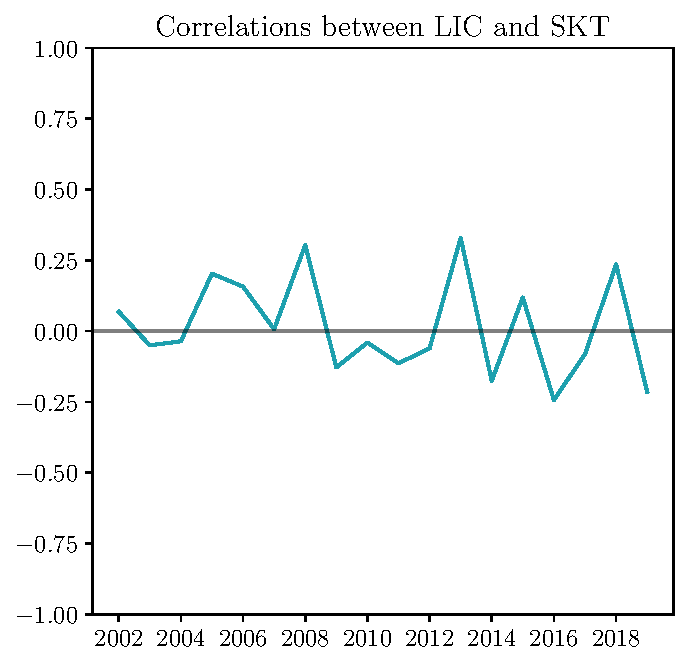
\includegraphics[width=0.9\textwidth]{images/week8/hres/corr_lic_skt_shortterm_temporal_anmomalous}
\caption{Temporal distribution of correlations of anomalous \gls{lilwet}  and \gls{skt}.}
\end{subfigure}
\caption{Correlations between \gls{lilwet}  and \gls{skt}. The left column contains correlations for raw data time-series and the right column contains the correlations for anomalous time-series. The top row contains correlations for individual time series. The bottom row contains pattern correlations between the two variables and how that changes over time.}
\label{fig:correlation_between_LIC_and_SKT.}
\end{figure}

\section[Regressions]{Regressions using temperature to predict Antarctic ice}
\label{sec:regressions_temp_ice}

\section[Statistics]{Statistics for Antarctic ice and temperature}

\section[Implications]{Implications for our understanding of Antarctic ice          }

\pagebreak
\section*{Things still to do for this Chapter}
\begin{enumerate}
    \item Correlations
    \item Temporal Aggregations
    \begin{itemize}
        \item Trend lines to ice.
        \item Remove total ice row for now (until we have volume data).
    \end{itemize}
    \item Regress temperature onto ice.
    \item Fill out red citation notes in the text.
    \item Generate relevant statistics.
    \item check comment made at the end of the mean distribution plots.
\end{enumerate}
\end{document}